\scanpage{38}
\margin{\figure{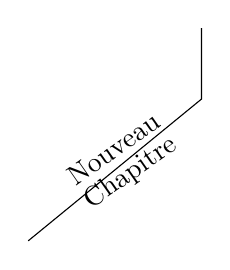
\begin{tikzpicture}\node[rotate=35] at (0,0) {\shortstack{Nouveau\\Chapitre}};\draw (-1.2,-1)--(1,.8)--(1,1.7);\end{tikzpicture}}}
1) Programme de la théorie de Dieudonné sur une base \inserted{$S$} où p est localement nilpotent.

 a) \uline{Foncteur de Dieudonné}. On \deleted{va} définiraun foncteur
\[
\diagram{\begin{tikzcd}
\underline D^*:\quad \mathrm{BT}(S)^0 \arrow[r] & \mathrm{Crisloclib}(S),
\end{tikzcd}}
\]
\margin{$\unsure{\mathbb D|D}^*$}
compatible aux images inverses (donc foncteur cartésien sur la catégorie fibrée des groupes de BT sur des bases où p est \unsure{loc.} nilp.). Si $S_0=\operatorname{Var}(p)$ on a une équivalence de catégories (cf.\qquad plus haut)
\[
\mathrm{Crisloclib}(S)\unsure{\approxeq|\simeq}\mathrm{Crisloclib}(S_0)
\]
de sorte que la donnée de $\underline D^*$ équivaut à la donnée de
\[
\diagram{\begin{tikzcd}
\underline D^*:\quad\mathrm{BT}(S_0)^0 \arrow[r] & \mathrm{Crisloclib}(S_0),
\end{tikzcd}}
\]
i.e. on est ramené \deleted{à la car. p.} au cas S de car. p. \deleted{\unsure{Pour connaitre, d}}
Dans le cas général, $\underline D^*(G)$ ne dépend que de $\deleted{\unsure{D^*}}G_0=G\times_S S_0$.

\deleted{\unsure{Utilis}} Plaçons nous sur $S_0$ de car. p. Utilisant $\underline f_G$ et $\underline V_G$ et la compatibilité de $\underline D^*$ aux images inverses, on voit que \deleted{le foncteur}
$\underline D^*(G_0)$ \deleted{peut}\inserted{$=M$} est naturellement muni de morphismes $F_M,V_M$ \deleted{satisfaisant}
\[
\diagram{\begin{tikzcd}
M^{(p)}=\underline f_S^*(M) \arrow[r,shift left,"F_M"] & M \arrow[l,shift left,"V_M"]
\end{tikzcd}}
\]
satisfaisant
\[
V_MF_M=p\operatorname{id}_M,\quad F_MV_M=p\operatorname{id}_{\unsure{M}}(p).
\]
On appelle un tel triple $(M,F_M,V_M)$ un (F-V-\uline{cristal}\inserted{ ou \uline{cristal de Dieudonné}}), et on a donc un foncteur
\[
\diagram{\begin{tikzcd}
\underline D^*:\quad\mathrm{BT}(S_0) \arrow[r] & \text{F-V-Cris}(S_0).
\end{tikzcd}}
\]
C'est ce foncteur qui mérite le nom de \uline{foncteur de Dieudonné}. On \deleted{\unsure{pouve|prouve}} \deleted{prouve que} voit que sa formation commute à tout changement de\inserted{ }base. De plus, on prouve que pour $S_0$ spectre d'un corps parfait, il coïncide \deleted{avec} à isomorphisme canonique près avec le foncteur de Dieudonné habituel, qui est alors une équivalence de catégories, de sorte que dans ce cas la
\margin{37}
